\documentclass[
  unicode,a4paper,9pt,
  % aspectratio=169,
  xcolor = {dvipsnames,svgnames},
  hyperref ={colorlinks=true,citecolor=Navy,linkcolor=NavyBlue,urlcolor=purple},
  ja=standard,lualatex
]{beamer}
\renewcommand{\baselinestretch}{1.4}

% ---fonts---
\PassOptionsToPackage{quiet}{fontspec}
\usefonttheme{serif}
\mathversion{bold}
\usepackage{luatexja-fontspec}
\setmainfont{TeX Gyre Termes}
\setmainjfont{Noto Sans CJK JP}
% \setmainjfont[BoldFont = HaranoAjiGothic-Regular]{HaranoAjiMincho}
% \setmainjfont[BoldFont = IPAGothic]{IPAMincho}
\setmathrm{Latin Modern Roman}
% \usepackage{newtxmath}

\usepackage{newunicodechar}
\newunicodechar{–}{-}

% ---refer `texdoc xcolor' at the command line---

% ---Display \subsubsection at the Index
% \setcounter{tocdepth}{3}

% ---Setting about the geometry of the document----
% \usepackage{a4wide}
% \pagestyle{empty}

% ---Physics and Math Packages---
\usepackage{amssymb,amsfonts,amsthm,mathtools}
\usepackage{physics,braket,bm,slashed}

% ---underline---
\usepackage[normalem]{ulem}

% ---cancel---
\usepackage{cancel}

% --- surround the texts or equations
\usepackage{fancybox,ascmac}

% ---settings of theorem environment---
\usepackage{amsthm}
\theoremstyle{definition}

% ---settings of proof environment---
\renewcommand{\proofname}{\textbf{証明}}
\renewcommand{\qedsymbol}{$\blacksquare$}

% ---Insert the figure (If insert the `draft' at the option, the process becomes faster.)---
\usepackage{graphicx}
% \usepackage{subcaption}

% ----Add a link to a text---
\usepackage{url,hyperref}
\usepackage{xcolor}

% ---Tikz---
\usepackage{tikz,pgf,pgfplots,circuitikz}
\pgfplotsset{compat=1.15}
\usetikzlibrary{intersections,arrows.meta,angles,calc,3d,decorations.pathmorphing,positioning}

% ---Add the section number to the equation, figure, and table number---
\makeatletter
   \renewcommand{\theequation}{\thesection.\arabic{equation}}
   \@addtoreset{equation}{section}
   
   \renewcommand{\thefigure}{\thesection.\arabic{figure}}
   \@addtoreset{figure}{section}
   
   \renewcommand{\thetable}{\thesection.\arabic{table}}
   \@addtoreset{table}{section}
\makeatother

% ---enumerate---
% \renewcommand{\labelenumi}{$\arabic{enumi}.$}
% \renewcommand{\labelenumii}{$(\arabic{enumii})$}

% ---beamer settings---
\usefonttheme{professionalfonts}
\usecolortheme{seahorse}
\setbeamercolor{structure}{fg=white}
\setbeamercolor{local structure}{fg=red}
\setbeamertemplate{itemize item}[ball]
\setbeamertemplate{enumerate item}[circle]
\setbeamercolor{bibliography entry author}{fg=black}
\setbeamercolor{bibliography item}{fg=black}
\setbeamercolor{alerted text}{fg=RoyalBlue}
\setbeamertemplate{frametitle continuation}{}
\setbeamertemplate{footline}[frame number]
\setbeamertemplate{navigation symbols}{} 
\setbeamersize{text margin left=10pt, text margin right=10pt}

% ---tcolorbox---
\usepackage{tcolorbox}
\tcbuselibrary{theorems}
\tcbuselibrary{raster}
\tcbuselibrary{skins}
\newtcolorbox{bluebox}[2][]{enhanced,
colframe=RoyalBlue!40!white,
colback=RoyalBlue!10!white,
coltitle=black,
drop fuzzy shadow, title={#2}
,#1}
\newtcolorbox{redbox}[2][]{enhanced,
colframe=DarkRed!40!white,
colback=DarkRed!10!white,
coltitle=black,
drop fuzzy shadow, title={#2}
,#1}

% ---tcolorbox---
\usepackage{tcolorbox}
\tcbuselibrary{raster,skins,breakable}
\newtcolorbox{graybox}[1][]{frame empty, colback=black!10!white, sharp corners}

% ---Ignore the Warnings---
\usepackage{silence}
\WarningFilter{latexfont}{Some font shapes}
\WarningFilter{latexfont}{Font shape}
\WarningFilter{latexfont}{Size substitutions}
\ExplSyntaxOn
\msg_redirect_name:nnn{hooks}{generic-deprecated}{none}
\ExplSyntaxOff

% ---Citation on the slides---
\newcommand*{\citefone}[2]{
  \begin{tikzpicture}[remember picture, overlay]
    \node[anchor=north east, align=left] at ($(current page.north east)-(0,0.0)$){
    {\tiny
      \cite{#1}
      #2
    }
    };
  \end{tikzpicture}

  \vspace*{-20pt}
}

\newcommand*{\citeftwo}[4]{
  \begin{tikzpicture}[remember picture, overlay]
    \node[anchor=north east, align=left] at ($(current page.north east)-(0,0.0)$){
    {\tiny
      \cite{#1}
      #2
    }
    \\[-2.4ex]
    {\tiny
      \cite{#3}
      #4
    }
    };
  \end{tikzpicture}

  \vspace*{-20pt}
}

\newcommand*{\citefthree}[6]{
  \begin{tikzpicture}[remember picture, overlay]
    \node[anchor=north east, align=left] at ($(current page.north east)-(0,0.0)$){
    {\tiny
      \cite{#1}
      #2
    }
    \\[-2.4ex]
    {\tiny
      \cite{#3}
      #4
    }
    \\[-2.4ex]
    {\tiny
      \cite{#5}
      #6
    }
    };
  \end{tikzpicture}

  \vspace*{-20pt}
}

\newcommand*{\citefonev}[3]{
  \begin{tikzpicture}[remember picture, overlay]
    \node[anchor=north east, align=left, text width=#3cm] at ($(current page.north east)-(0,0.0)$){
    {{\fontsize{5pt}{0pt}\selectfont
      \cite{#1}
      #2\par}
    }
    };
  \end{tikzpicture}

  \vspace*{-20pt}
}

\newcommand*{\citeftwov}[5]{
  \begin{tikzpicture}[remember picture, overlay]
    \node[anchor=north east, align=left, text width=#5cm] at ($(current page.north east)-(0,0.0)$){
    {{\fontsize{5pt}{0pt}\selectfont
      \cite{#1}
      #2\par}

      {\fontsize{5pt}{0pt}\selectfont
      \cite{#3}
      #4\par}
    }
    };
  \end{tikzpicture}

  \vspace*{-20pt}
}

\newcommand*{\citefthreev}[7]{
  \begin{tikzpicture}[remember picture, overlay]
    \node[anchor=north east, align=left, text width=#7cm] at ($(current page.north east)-(0,0.0)$){
    {{\fontsize{5pt}{0pt}\selectfont
    \cite{#1}
    #2\par}

    {\fontsize{5pt}{0pt}\selectfont
    \cite{#3}
    #4\par}

    {\fontsize{5pt}{0pt}\selectfont
    \cite{#5}
    #6\par}
    }
    };
  \end{tikzpicture}

  \vspace*{-20pt}
}


% ---Title---
\title{
  title
}
\author{
  author
}
\date{Last modified: \today}

\begin{document}

\begin{frame}

  \setbeamertemplate{blocks}[rounded][shadow=true]
  \setbeamercolor{block body}{bg=RoyalBlue!10!white, fg=black}
  \begin{block}{}
    \vspace*{5pt}

    \centering\Large
    Spontaneous R-symmetry breaking in O'Raifeartaigh models
    \\
    \normalsize
    David Shih.
    \\
    \small
    \href{https://doi.org/10.1088/1126-6708/2008/02/091}{JHEP 02 (2008) 091},
    \href{https://arxiv.org/abs/hep-th/0703196}{arXiv:hep-th/0703196}.

    \vspace*{5pt}
  \end{block}

  \vspace*{1cm}

  \begin{center}
    安倍研 M1 宮根一樹\\
    2024 6/20 (木)
  \end{center}

\end{frame}

\nocite{Shih:2007av}

\begin{frame}
  \frametitle{読んだ動機など}
  \citefone{Nelson:1993nf}{A. E. Nelson and N. Seiberg, Nucl. Phys. B 416 (1994) 46-62.}

  \begin{center}
    「現在行っているモジュライ固定の研究に、R対称性の観点から何か言えるかもしれない」
  \end{center}
  というお話があった。

  これは、1994年にNelsonとSeibergが主張したこと\cite{Nelson:1993nf}で以下の通り:
  \begin{center}
    「\textcolor{DarkMagenta}{R対称性}が破れている」
    $\implies$
    「\textcolor{Goldenrod}{超対称}が自発的に破れている」
  \end{center}

  \begin{figure}
    \centering
    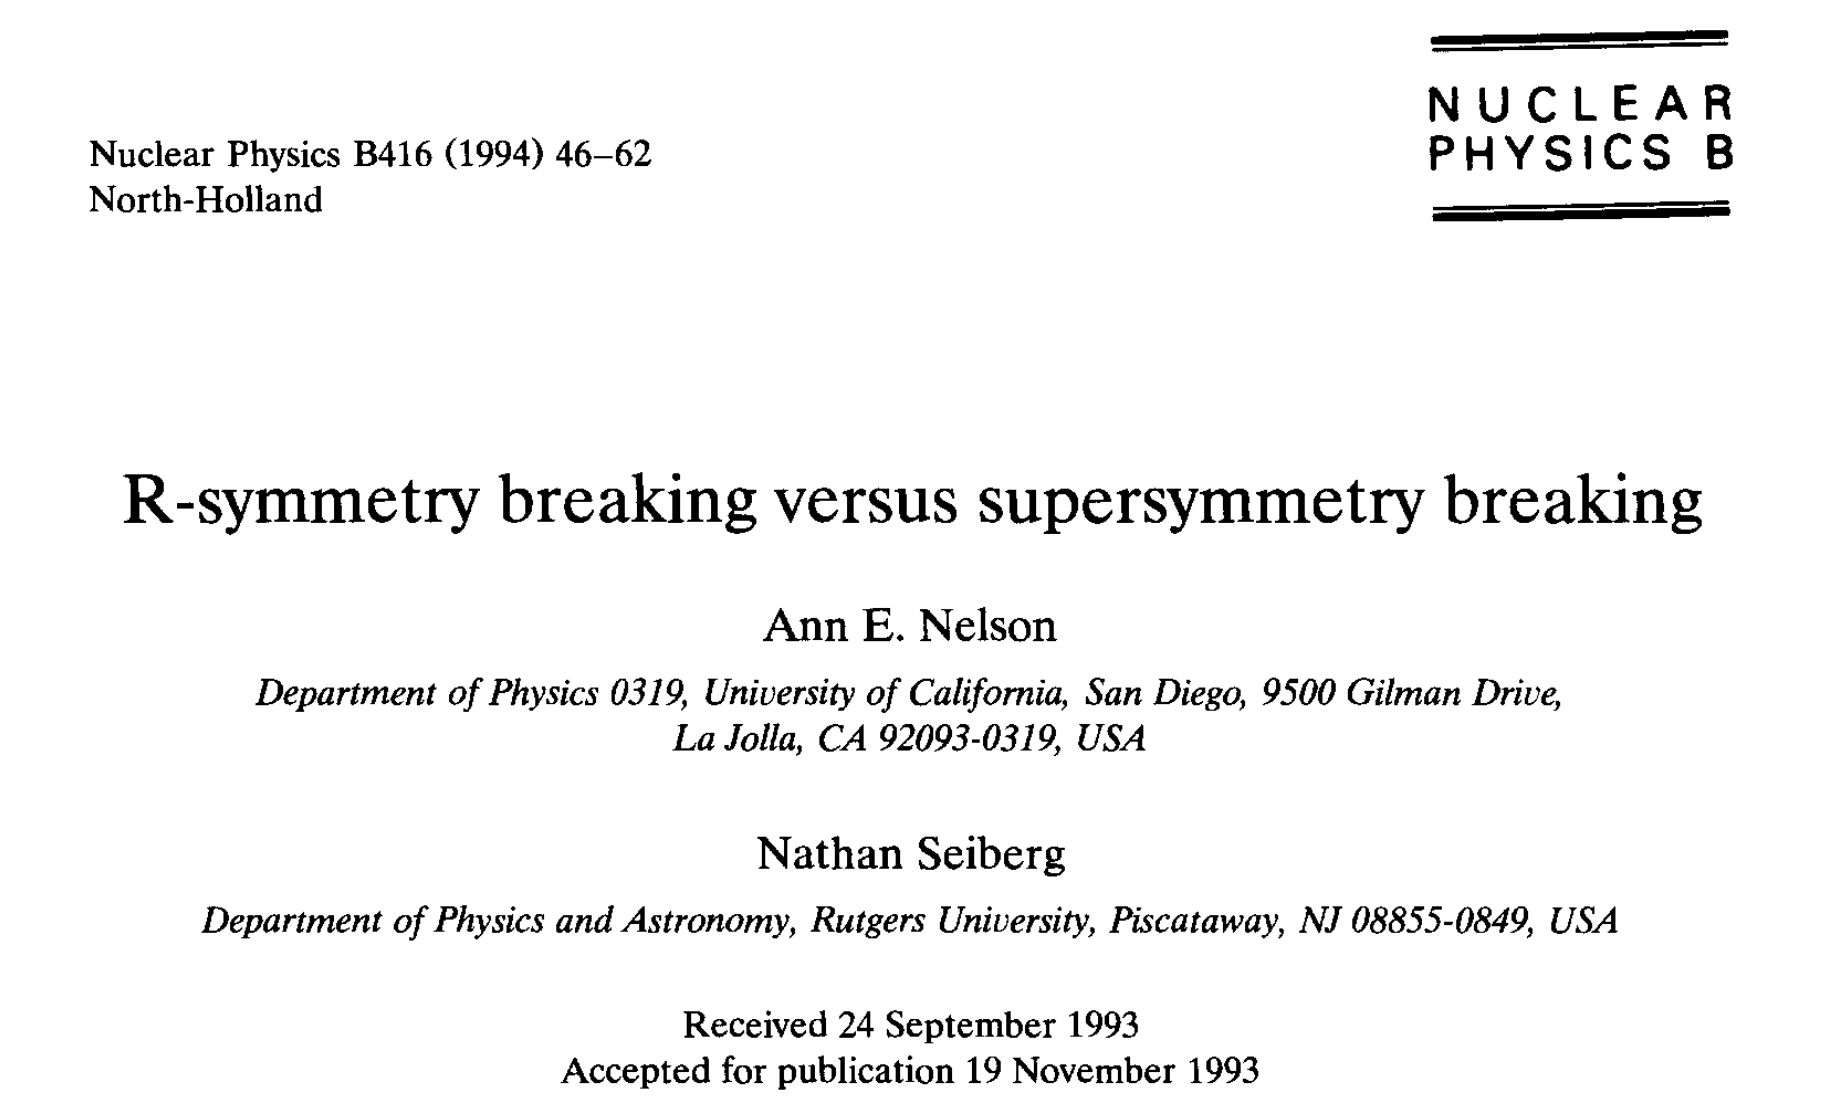
\includegraphics[width=0.6\textwidth]{fig/Nelson1993nf.PNG}
  \end{figure}

  \begin{center}
    (安倍研のActivityで紹介したものです。)
  \end{center}

\end{frame}

\begin{frame}
  \citefone{Shih:2007av}{D. Shih, JHEP 02 (2008) 091}
  \setbeamertemplate{blocks}[rounded][shadow=true]
  \setbeamercolor{block body}{bg=red!10!white, fg=black}
  \begin{block}{}
    \centering
    「\textcolor{DarkMagenta}{R対称性}の破れ」
    $\implies$
    「\textcolor{Goldenrod}{超対称の破れ}」
  \end{block}

  先ほど紹介した論文に関連して、以下の論文を読む\cite{Shih:2007av}。

  \begin{figure}
    \centering
    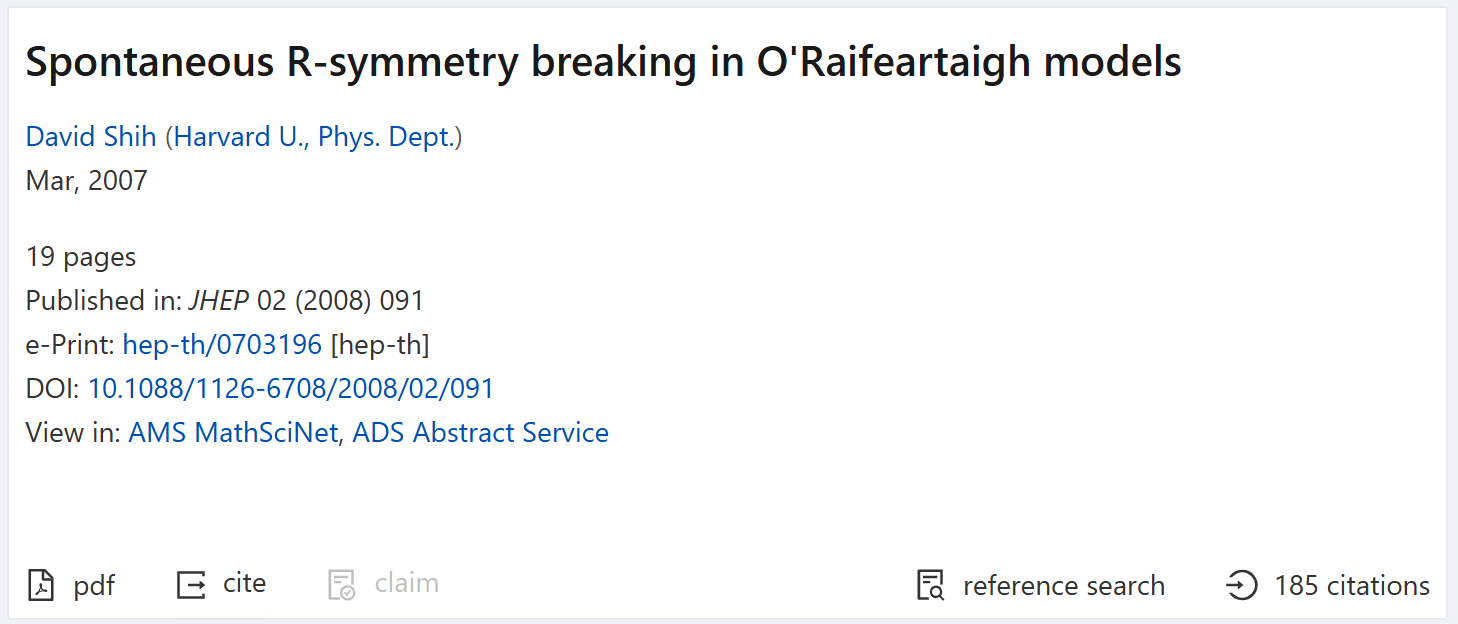
\includegraphics[width=0.6\textwidth]{fig/Shih2007av.PNG}
  \end{figure}

  \uline{論文の概要}

  \begin{itemize}
    \item
          Nelson\ \& Seibergによれば、SUSYを破るためには、(R対称性を理論がもっているなら)それを破らなくてはならない。
    \item
          この論文では、\textcolor{FireBrick}{モデルの摂動ダイナミクス自体}(量子補正)でR対称性を破ることを考える。
    \item
          また、R電荷に条件がつくことが分かる。
  \end{itemize}

\end{frame}

% ----------------------------------------------------------------------------------------------

\section{イントロダクション}

\begin{frame}[plain]
  \huge \secname
\end{frame}


\subsection{自発的対称性の破れ}

\begin{frame}
  \frametitle{\subsecname}

  $n$個の場$\textcolor{DarkGreen}{\Phi_{i}(x)}$が作るポテンシャル$V(\textcolor{DarkGreen}{\Phi_{1},\cdots,\Phi_{n}})$の極小値に興味がある。

  その極小な点(準安定点)を真空$\textcolor{RoyalBlue}{\ev*{\Phi_{i}}}$といい、その真空からの揺らぎ$\textcolor{FireBrick}{\tilde{\Phi}_{i}}$を考える。
  \begin{equation}
    \textcolor{DarkGreen}{\Phi_{i}}
    =
    \textcolor{RoyalBlue}{\ev*{\Phi_{i}}}+\textcolor{FireBrick}{\tilde{\Phi}_{i}}
    \nonumber
  \end{equation}

  この揺らぎに対してのポテンシャル$\tilde{V}$は、元のポテンシャル$V$の対称性を保っているとは限らない。
  \begin{equation}
    \tilde{V}(\textcolor{FireBrick}{\tilde{\Phi}_{i}})
    =
    V(\textcolor{RoyalBlue}{\ev*{\Phi_{i}}}+\textcolor{FireBrick}{\tilde{\Phi}_{i}})
    \nonumber
  \end{equation}
  \begin{center}
    $\longrightarrow$\ 「対称性が自発的に破れている」という。
  \end{center}

  \pause

  もし、場の真空期待値が$0\ (\textrm{i.e.\ } \ev*{\Phi_{i}}=0)$なら、(tree levelでは)対称性は保たれる。
  \begin{equation}
    \tilde{V}(\tilde{\Phi}_{i})
    =
    V(\textcolor{gray}{\ev*{\Phi_{i}}+}\tilde{\Phi}_{i})
    。
    \nonumber
  \end{equation}

\end{frame}


\subsection{超対称性}

\begin{frame}
  \frametitle{\subsecname}

  カイラル多重項$\Phi=\{\phi,\psi,F\}$。この多重項に含まれている粒子の間を
  \begin{equation}
    \textcolor{DarkMagenta}{\xi Q}\phi
    =
    \sqrt{2}\xi \psi
    \ ,\quad
    \textcolor{DarkMagenta}{\xi Q}\psi
    =
    i\sqrt{2}\sigma^{\mu}\bar{\xi}\partial_{\mu}\phi
    +
    \sqrt{2}\xi F
    \ ,\quad
    \textcolor{DarkMagenta}{\xi Q}F
    =
    i\sqrt{2}\bar{\xi}\bar{\sigma}^{\mu}\partial_{\mu}\psi
    \nonumber
  \end{equation}
  のように変換するのが、(無限小)\textcolor{Goldenrod}{超対称変換}。

  この変換で不変な理論のことを\textcolor{Goldenrod}{超対称な理論}と言う。

  \vspace*{15pt}

  また、超対称性を考えるときに、反可換な座標$\theta$を用いた超場形式を用いると、ミンコフスキー時空とグラスマン座標$\theta$を合わせた超空間$(x^{\mu},\theta,\bar{\theta})$が超対称変換の表現空間となっている。
  \begin{gather}
    \Phi
    =
    \phi(x)+i\theta\sigma^{\mu}\bar{\theta}\partial_{\mu}\phi(x)+\frac{1}{4}\theta\theta\overline{\theta\theta}\partial^{2}\phi(x)
    \nonumber
    \\
    \hspace*{1.5cm}
    +\sqrt{2}\theta\psi(x)-\frac{i}{\sqrt{2}}\theta\theta\partial_{\mu}\psi\sigma^{\mu}\bar{\theta}+\theta\theta F(x)
    \nonumber
    \\
    Q_{\alpha}
    =
    \pdv{}{\theta^{\alpha}}
    -
    i\sigma_{\alpha\dot{\alpha}}^{\mu}\partial_{\mu}
    \nonumber
  \end{gather}

\end{frame}

\begin{frame}

  超場によって構成される以下のポテンシャルを考えると超対称な理論が得られる。
  \begin{itemize}
    \item
          \uline{$W$:超ポテンシャル} $\ \rightarrow\ $ 超場の正則な関数で書かれたもの。
    \item
          \uline{$K$:ケーラーポテンシャル} $\ \rightarrow\ $ 実超場によって書かれたもの。
  \end{itemize}

  ラグランジアンは$W, K$に含まれているグラスマン座標を積分して取り除くことで得られる。
  \begin{equation}
    \mathcal{L}
    =
    \int\dd^4\theta\ K(\Phi,\Phi^{\dag})
    +
    \left[
      \int\dd^2 \theta\ W(\Phi)
      +
      \textrm{h.c.}
      \right]
    \nonumber
  \end{equation}

  この方法で得られたラグランジアンで、運動項を除いた項をポテンシャルとして扱う。

\end{frame}


\subsection{今回考える理論 (O'Raifeartaigh模型)}

\begin{frame}
  \frametitle{\subsecname}

  次の理論を考える。
  \begin{equation}
    \left\{
    \begin{alignedat}{1}
      W
      &=
      fX
      +
      \frac{1}{2}(M_{ij}+XN_{ij})\phi_{i}\phi_{j}
      \\
      K
      &=
      X^{\dag}X
      +
      \phi^{\dag}_{i}\phi_{i}
    \end{alignedat}
    \right.
    \nonumber
  \end{equation}
  ただし、$X,\phi_{i}$はいずれもカイラル超場。

  この理論が次の変換で不変であることを仮定する(\textcolor{DarkRed}{R対称性})
  \begin{equation}
    X\rightarrow e^{2i\alpha}X
    \ ,\quad
    W\rightarrow e^{2i\alpha}W
    \nonumber
  \end{equation}
  (上の仮定から$\phi_{i}\rightarrow e^{iq_{i}\alpha}\phi_{i}$と変換したときの$q_{i}$が決まってくる。が、後で。)

  この理論の真空は
  \begin{equation}
    V_{0}=f^2
    \ ,\quad
    \ev*{\phi_{i}}
    =
    0
    \ ,\quad
    \ev*{X}
    =
    \textrm{\ 任意の定数\ }
    \nonumber
  \end{equation}

  $X$の真空期待値は任意(擬モジュライ)なので、$\ev*{X}=0$とすればR対称性は保たれてしまう。(\uline{c.f.}\ $\ev*{\Phi_{i}}=0$なら$\tilde{V}(\tilde{\Phi}_{i})=V(\textcolor{gray}{\ev*{\Phi_{i}}+}\tilde{\Phi}_{i})$。)

\end{frame}


\subsection{今回の論文の目的}


\begin{frame}
  \frametitle{\subsecname}

  したがって、\uwave{場$X$について}はポテンシャルが\textcolor{red}{立ち上がらない}。
  \begin{equation}
    V(X)
    =
    V_{0}
    +
    \textcolor{gray}{m_{X}^2}|X|^2
    +
    \mathcal{O}(|X|^4)
    \nonumber
  \end{equation}

  \pause

  そこで、今回は
  \setbeamertemplate{blocks}[rounded][shadow=true]
  \setbeamercolor{block body}{bg=red!10!white, fg=black}
  \begin{block}{}
    \centering
    量子補正(Coleman-Weinbergポテンシャル)で$m_{X}^2$を計算\\
    ${\big \Downarrow}$\\
    R対称性を自発的に破る
  \end{block}
  ことを考える。

  \begin{itemize}
    \item
          R対称性が自発的に破れるためには、$m_{X}^2$の符号が負であることが必要\\
          $\ \longrightarrow\ $ $\phi_i$のR電荷$q_{i}$に条件がつく。
    \item
          論文では、$|X|^4$の係数が計算されていなかった。\\
          具体例のときに、正であることは確認。が、一般にそうなっている?
  \end{itemize}

\end{frame}

\section{本論}

\begin{frame}[plain]
  \huge \secname
\end{frame}


\subsection{超対称性の破れ}

\begin{frame}
  \frametitle{\subsecname}

  今回考える理論。
  \begin{equation}
    W
    =
    fX
    +
    \frac{1}{2}(M_{ij}+XN_{ij})\phi_{i}\phi_{j}
    \nonumber
  \end{equation}

  $M,N$は複素対称行列。$\det M\neq 0$、$f> 0$を仮定。

  また、$M$を次の形で書く。$M_{i}$はR電荷が$q_{i}$の場の質量行列。(\hyperref[eqn:eg]{具体例})
  \begin{equation}
    M
    =
    \begin{pmatrix}
                &           &       &       &       & M_{1} \\
                &           &       &       & M_{2} &       \\
                &           &       & \cdot &       &       \\
                &           & \cdot &       &       &       \\
                & M_{2}^{T} &       &       &       &       \\
      M_{1}^{T} &           &       &       &       &
    \end{pmatrix}
    \nonumber
  \end{equation}

  R対称性を課すと、R電荷に条件がつく。
  \begin{equation}
    M_{ij}\neq 0
    \implies
    R(\phi_{i})+R(\phi_{j})=2
    \ ,\quad
    N_{ij}\neq 0
    \implies
    R(\phi_{i})+R(\phi_{j})=0
    \nonumber
  \end{equation}

\end{frame}

\begin{frame}

  $F$-termのSUSY条件は
  \begin{equation}
    \pdv{W}{\phi_{i}}
    =
    0
    \implies
    (M_{ij}+XN_{ij})\phi_{j}
    =
    0
    \quad
    (j=1,\cdots,n)
    \nonumber
  \end{equation}

  方程式を満たす$\ev*{\phi_{i}}(\neq 0)$が存在するかどうか$\ \rightarrow\ \det(M+XN)$を計算\\
  (\uline{c.f.}\ $\det\exp A=\exp\tr A$)
  \begin{align}
    \det (M+XN)
     & =
    \exp\left[ \Tr\ln (1+XM^{-1}N) \right]\det M
    \nonumber
    \\
     & =
    \exp\left[
      -\sum_{k=1}^{\infty}\frac{(-X)^{k}}{k}\Tr(M^{-1}N)^{k}
      \right]
    \det M
    \nonumber
    \\
     &
    =
    \det M\neq 0
    \nonumber
  \end{align}
  最後の等式は\uwave{R電荷の条件}から$\Tr (M^{-1}N)$が$0$となることを用いている。
  \begin{equation}
    \left(
    M_{ij}\neq 0
    \implies
    R(\phi_{i})+R(\phi_{j})=2
    \ ,\quad
    N_{ij}\neq 0
    \implies
    R(\phi_{i})+R(\phi_{j})=0
    \right)
    \nonumber
  \end{equation}
  この関係から、R対称性を課すと$M^{-1}N$を計算するときに$M$か$N$の成分が必ず消えている。

  \begin{center}
    {\Huge $\Downarrow$}\\
    よって、非自明な超対称性を破る真空は存在しない。
  \end{center}

\end{frame}


\subsection{\texorpdfstring{$m_{X}^2$}{mX2}の計算}

\begin{frame}
  \frametitle{\subsecname}

  Coleman-Weinbergポテンシャルを展開して、$|X|^2$の係数を探る。
  \begin{equation}
    V_{\textrm{eff}}^{(1)}
    =
    \frac{1}{64\pi^2}
    \Tr (-1)^{F}
    \mathcal{M}^{4}\ln\frac{\mathcal{M}^2}{\Lambda^{2}}
    \nonumber
  \end{equation}
  $\Tr (-1)^{F}$は超トレース。$\mathcal{M}$は、スカラーかフェルミオンの質量行列で
  \begin{align}
    \mathcal{M}_{B}^2
     & =
    \begin{pmatrix}
      W^{\dag}_{ik}W^{kj} & W^{\dag}_{ijk}W^{k} \\
      W^{ijk}W_{k}^{\dag} & W^{ik}W_{kj}^{\dag}
    \end{pmatrix}
    =
    (\hat{M}+X\hat{N})^2+f\hat{N}
    \nonumber
    \\
    \mathcal{M}_{F}^2
     & =
    \begin{pmatrix}
      W^{\dag}_{ik}W^{kj} & 0                   \\
      0                   & W^{ik}W_{kj}^{\dag}
    \end{pmatrix}
    =
    (\hat{M}+X\hat{N})^2
    \nonumber
  \end{align}
  ただし、$W_{i}\equiv\partial W/\partial\phi_{i}$。これがスカラーやフェルミオンの質量行列というのは、

\end{frame}


\begin{frame}

  ここで、ポテンシャルの公式を書き換える。
  \begin{equation}
    \frac{1}{64\pi^2}
    \Tr (-1)^{F}
    \mathcal{M}^{4}\ln\frac{\mathcal{M}^2}{\Lambda^{2}}
    =
    -\frac{1}{32\pi^2}
    \Tr\int^{\Lambda}_{0}\dd v\
    v^5\left( \frac{1}{v^2+\mathcal{M}_{B}^2}-\frac{1}{v^2+\mathcal{M}_{F}^2} \right)
    \nonumber
  \end{equation}

  ---------------------------------------------------------------------------------

  積分の部分は以下のようになっている。
  \begin{equation}
    \int\dd v\
    \frac{v^5}{v^2+\mathcal{M}^2}
    =
    -\frac{1}{2}\mathcal{M}^2 v^2
    +
    \frac{1}{4}v^4
    +
    \frac{1}{2}\mathcal{M}^4\ln(\mathcal{M}^2+v^2)
    \nonumber
  \end{equation}

  あとは$\ln \Lambda^2$で発散する項をみて
  \begin{align}
    \left[
      \frac{1}{2}\mathcal{M}^4\ln(\mathcal{M}^2+v^2)
      \right]_{0}^{\Lambda}
     & =
    \frac{1}{2}\mathcal{M}^4\ln\left( 1+\frac{\Lambda^2}{\mathcal{M}^2} \right)
    \nonumber
    \\
     & \sim
    -
    \frac{1}{2}\mathcal{M}^4\ln\frac{\mathcal{M}^2}{\Lambda^2}
    \nonumber
  \end{align}

  こんな感じなのではないかと思います。

\end{frame}

\begin{frame}

  分母に$X$がいるので、これについて展開\ $\rightarrow$\ $2$次の係数を拾ってそれを$m_{X}^2$とする。
  \begin{align}
    \int^{\Lambda}_{0}\dd v\
    \frac{v^5}{v^2+\mathcal{M}_{B}^2}
     & =
    \int^{\Lambda}_{0}\dd v\
    \frac{v^5}{v^2+\hat{M}^2+f\hat{N}+\{\hat{M},\hat{N}\}X+\hat{N}^2X^2}
    \nonumber
    \\
     & \hspace*{-2cm}\rightarrow
    \int^{\Lambda}_{0}\dd v\
    \frac{v^5}{v^2+\hat{M}^2+f\hat{N}}
    \left\{
    -
    \frac{1}{v^2+\hat{M}^2+f\hat{N}}
    \hat{N}^2
    \right.
    \nonumber
    \\
     & \left.
    +
    \frac{1}{v^2+\hat{M}^2+f\hat{N}}\{\hat{M},\hat{N}\}
    \frac{1}{v^2+\hat{M}^2+f\hat{N}}\{\hat{M},\hat{N}\}
    \right\}
    X^2
    \nonumber
  \end{align}

  ここで、部分積分をすると、$m_{X}^2$への寄与は
  \begin{equation}
    \frac{1}{16\pi^2}\Tr\int_{0}^{\Lambda}\dd v
    \frac{v^3}{v^2+\hat{M}^2+f\hat{N}}
    \left(
    \hat{N}^2
    -
    \frac{1}{2}\{\hat{M},\hat{N}\}\frac{1}{v^2+\hat{M}^2+f\hat{N}}\{\hat{M},\hat{N}\}
    \right)
    \nonumber
  \end{equation}

  フェルミオンの寄与も同様に計算する。すると、最終的に
  \begin{align}
    m_{X}^2
     & =
    \frac{1}{16\pi^2}\Tr\int_{0}^{\Lambda}\dd v
    \nonumber
    \\
     & \hspace*{1cm}
    \times
    \left[
      \frac{v^3}{v^2+\hat{M}^2+f\hat{N}}
      \left(
      \hat{N}^2
      -
      \frac{1}{2}\{\hat{M},\hat{N}\}\frac{1}{v^2+\hat{M}^2+f\hat{N}}\{\hat{M},\hat{N}\}
      \right)
      \right.
      \nonumber
    \\
     & \hspace*{1.2cm}
      \left.
      -\frac{v^3}{v^2+\hat{M}^2}
      \left(
      \hat{N}^2
      -
      \frac{1}{2}\{\hat{M},\hat{N}\}\frac{1}{v^2+\hat{M}^2}\{\hat{M},\hat{N}\}
      \right)
      \right]
    。
    \nonumber
  \end{align}
\end{frame}

\begin{frame}

  ここで、次のような関数を用意する。
  \begin{equation}
    \mathcal{F}(v)
    \equiv
    \left( v^2+\hat{M}^2 \right)^{-1}
    \cdot
    f\hat{N}
    \nonumber
  \end{equation}

  これを用いれば、$m_{X}^2$は次のように書ける。
  \begin{equation}
    m_{X}^2
    =
    \frac{1}{16\pi^2 f^2}
    \int_{0}^{\infty}\dd v\ v^3\Tr
    \left[
      \frac{\mathcal{F}(v)^4}{1-\mathcal{F}(v)^2}v^2
      -
      2\left( \frac{\mathcal{F}(v)^2}{1-\mathcal{F}(v)^2}\hat{M} \right)^2
      \right]
      \tag*{\heartsuit}
    \label{eqn:mX2_Fv}
  \end{equation}

  式の形をみて、
  \begin{gather}
    M_{1}^2
    =
    \frac{1}{16\pi^2 f}\int_{0}^{\infty}\dd v\ v^5\Tr\left[ \frac{\mathcal{F}(v)^4}{1-\mathcal{F}(v)^2} \right]
    \nonumber
    \\
    M_{2}^2
    =
    \frac{1}{8\pi^2 f}\int_{0}^{\infty}\dd v\ v^3\Tr\left[ \left( \frac{\mathcal{F}(v)^2}{1-\mathcal{F}(v)^2}\hat{M}  \right)^2 \right]
    \nonumber
    \\
    m_{X}^2=M_{1}^2-M_{2}^2
    \nonumber
  \end{gather}
  としておく。これで、$m_{X}^2$に関する公式が得られたことになる。Appendixで具体的なモデルに対してこの公式を適用している。

\end{frame}


\subsection{\texorpdfstring{$m_{X}^2$}{mX2}とR電荷の関係}

\begin{frame}
  \frametitle{\subsecname}

  ここでは、この公式とR電荷との関係を見てみる。
  \begin{gather}
    m_{X}^2=M_{1}^2-M_{2}^2
    \nonumber
    \\
    M_{2}^2
    =
    \frac{1}{8\pi^2 f}\int_{0}^{\infty}\dd v\ 
    v^3\Tr\left[ \left( \frac{\mathcal{F}(v)^2}{1-\mathcal{F}(v)^2}\hat{M}  \right)^2 \right]
    \nonumber
  \end{gather}

  分かることは
  \begin{center}
    もし、全ての場$\phi_{i}$のR電荷が$0$か$2$ \\
    ${\Big \Downarrow}$ \\
    $M_{2}^2=0$となって$m_{X}^2=M_{1}^2>0$となる。
  \end{center}

  したがって、
  \setbeamertemplate{blocks}[rounded][shadow=true]
  \setbeamercolor{block body}{bg=Goldenrod!10!white, fg=black}
  \begin{block}{}
    \centering
    量子補正で$\ev*{X}\neq 0$としたいんだったら \\
    R電荷が$0$か$2$以外の場の存在が必要。
  \end{block}

\end{frame}


\begin{frame}



  

\end{frame}


\subsection{簡単な模型での計算}

\begin{frame}
  \frametitle{\subsecname}

  以上の視点で、簡単な模型を考察する。
  \begin{equation}
    W=\lambda X\phi_{1}\phi_{2}+m_{1}\phi_{1}\phi_{3}+\frac{1}{2}m_{2}^2\phi_{2}^2+fX
    \nonumber
  \end{equation}

  「R電荷が0と2のものを含まない模型」という意味で一番シンプル。
  $$
    R_{X}=2\ , \quad R(\phi_{1})=-1\ , \quad R(\phi_{2})=1\ ,\quad R(\phi_{3})=3
  $$

  ポテンシャルは
  \begin{align}
    V
     & =
    \bar{F}^{X}F^{X}
    +
    \bar{F}^{\phi_{1}}F^{\phi_{1}}
    +
    \bar{F}^{\phi_{2}}F^{\phi_{2}}
    +
    \bar{F}^{\phi_{3}}F^{\phi_{3}}
    \nonumber
    \\
     & =
    |\lambda X\phi_{2}+m_{1}\phi_{3}|^2
    +
    |\lambda X\phi_{1}+m_{2}\phi_{2}|^2
    +
    |m_{1}\phi_{1}|^2
    +
    |\lambda \phi_{1}\phi_{2}+f|^2
    \nonumber
  \end{align}

  (ここで、カイラル超場$\Phi(=\phi_{i}\textrm{\ or\ }X)$のスカラーを同じ記号$\Phi$で書いている。)

\end{frame}

\begin{frame}

  次の記述が分かりませんでした。
  \begin{figure}
    \centering
    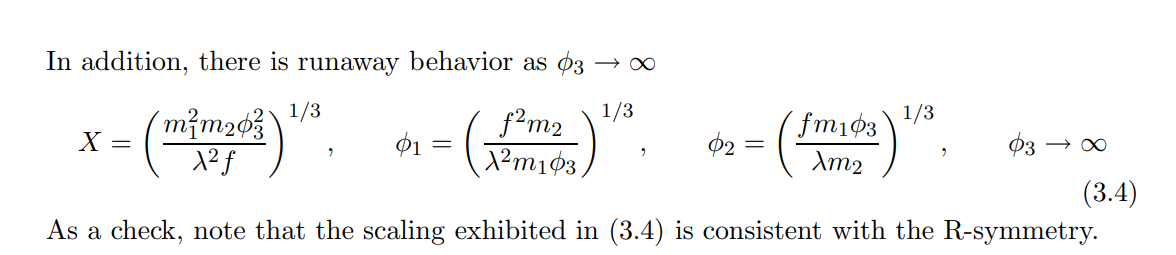
\includegraphics[width=0.9\textwidth]{fig/Shih2007avq1.PNG}
  \end{figure}

  一応、ポテンシャルを微分すると以下。
  \begin{align}
    \left\{
    \begin{alignedat}{1}
      V_{X}
      & =
      \lambda\phi_{2}(\lambda\bar{X}\bar{\phi}_{2}+m_{1}\bar{\phi}_{3})
      +
      \lambda\phi_{1}(\lambda\bar{X}\bar{\phi}_{1}+m_{2}\bar{\phi}_{2})
      \nonumber
      \\
      V_{\phi_{1}}
      & =
      \lambda\phi_{2}(\lambda\bar{\phi}_{1}\bar{\phi}_{2}+f)
      +
      \lambda X(\lambda\bar{X}\bar{\phi}_{1}+m_{2}\bar{\phi}_{2})
      +
      m_{1}^{2}\bar{\phi}_{1}
      \nonumber
      \\
      V_{\phi_{2}}
      & =
      \lambda\phi_{1}(\lambda\bar{\phi}_{1}\bar{\phi}_{2}+f)
      +
      \lambda\bar{X}(\lambda\bar{X}\bar{\phi}_{2}+m_{1}\bar{\phi}_{3})
      +
      m_{2}(\lambda\bar{X}\bar{\phi}_{1}+m_{2}\bar{\phi}_{2})
      \nonumber
      \\
      V_{\phi_{3}}
      & =
      m_{1}(\lambda \bar{X}\bar{\phi}_{2}+m_{1}\bar{\phi}_{3})
      \nonumber
    \end{alignedat}
    \right.
    \nonumber
  \end{align}

\end{frame}

\begin{frame}

  続き
  \begin{figure}
    \centering
    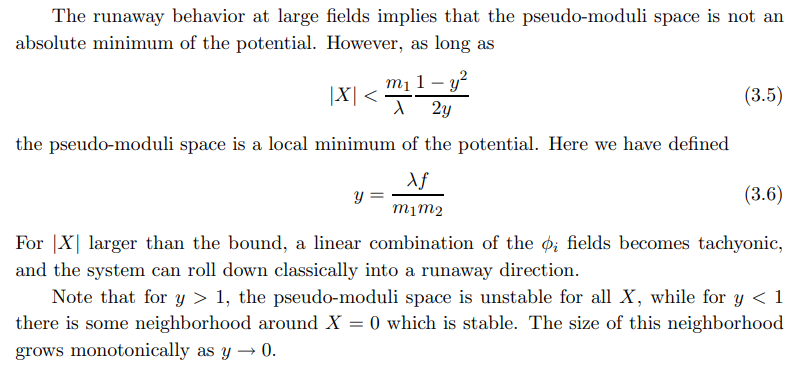
\includegraphics[width=0.9\textwidth]{fig/Shih2007avq2.PNG}
  \end{figure}

  ここで定義された$y$は、$X$の安定性を表す指標になる。($y<1$だと安定)

\end{frame}

\begin{frame}

  今回の質量行列などは以下の通り。
  \begin{gather}
    W=\lambda X\phi_{1}\phi_{2}+m_{1}\phi_{1}\phi_{3}+\frac{1}{2}m_{2}^2\phi_{2}^2+fX
    \label{eqn:eg}
    \nonumber
    \\
    M
    =
    \begin{pmatrix}
      0     & 0     & m_{1} \\
      0     & m_{2} & 0     \\
      m_{1} & 0     & 0     \\
    \end{pmatrix}
    \ ,\quad
    N
    =
    \begin{pmatrix}
      0       & \lambda & 0 \\
      \lambda & 0       & 0 \\
      0       & 0       & 0
    \end{pmatrix}
    \nonumber
  \end{gather}

  これを$\mathcal{F}(v)$を求め、$M_{1}^2, M_{2}^2$を計算する。
  \begin{align}
    \mathcal{F}(v)
     & =
    \left( v^2+\hat{M}^2 \right)^{-1}
    \cdot
    f\hat{N}
    \nonumber
    \\
     & =
    \begin{pmatrix}
      0 & 0                     & 0                     & 0                     & f\lambda /m_{1}^2+v^2 & 0 \\
      0 & 0                     & 0                     & f\lambda /m_{2}^2+v^2 & 0                     & 0 \\
      0 & 0                     & 0                     & 0                     & 0                     & 0 \\
      0 & 0                     & f\lambda /m_{1}^2+v^2 & 0                     & 0                     & 0 \\
      0 & f\lambda /m_{2}^2+v^2 & 0                     & 0                     & 0                     & 0 \\
      0 & 0                     & 0                     & 0                     & 0                     & 0 \\
    \end{pmatrix}
    \nonumber
  \end{align}

\end{frame}

\begin{frame}

  この$\mathcal{F}(v)$から$M_{1}^2, M_{2}^{2}$を計算して、先ほどの$y=\lambda f/m_{1}m_{2}$で展開する。
  \begin{align}
    M_{1}^2
     & =
    \frac{m_{1}^2\lambda^2}{8\pi^2}
    \frac{-4r^2\ln r+r^4-1}{(r^2-1)^3}
    y^2
    +
    \mathcal{O}(y^4)
    \nonumber
    \\
    M_{2}^2
     & =
    \frac{m_{1}^2\lambda^2}{4\pi^2}
    \frac{r^4\left\{ (r^2+1)\ln r-r^2+1 \right\}}{(r^2-1)^3}
    y^2
    +
    \mathcal{O}(y^4)
    \nonumber
  \end{align}

  よって
  \begin{equation}
    m_{X}^2
    =
    -
    \frac{m_{1}^2\lambda^2 y^2}{8\pi^2}
    \dfrac{r^2 \left\{ 2r^2(r^2+3)\ln r-(3r^4-2r^2-1) \right\}}{(r^2-1)^3}
    +
    \mathcal{O}(y^4)
    \nonumber
  \end{equation}

  \begin{figure}
    \centering
    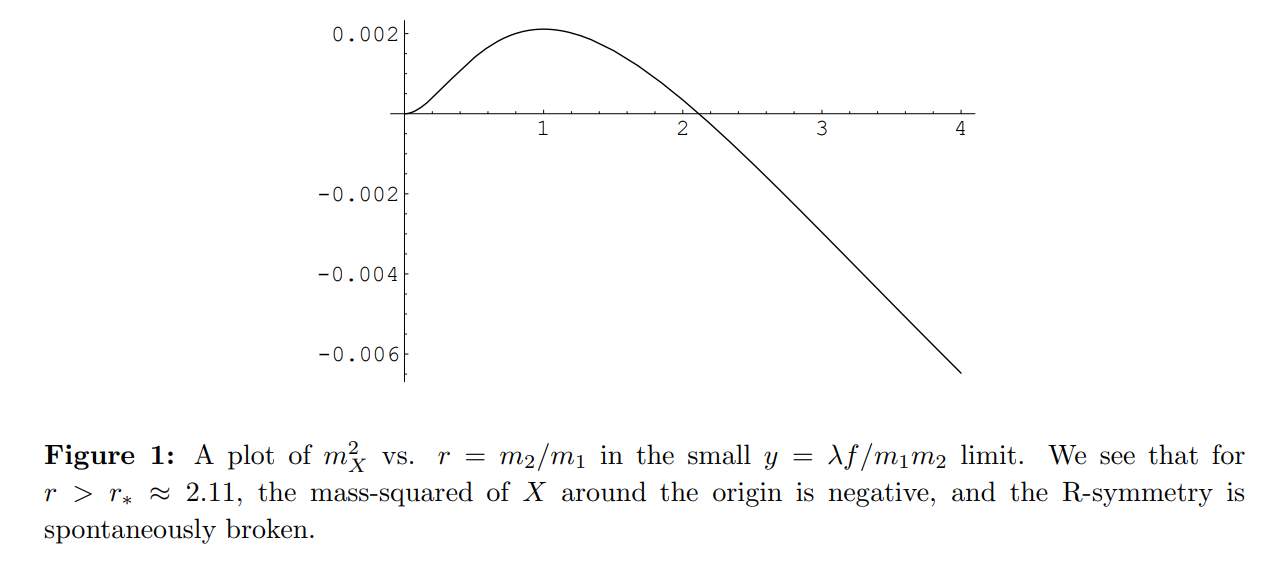
\includegraphics[width=0.9\textwidth]{fig/Shih2007avfig.PNG}
  \end{figure}

\end{frame}

\begin{frame}

  \begin{itemize}
    \item
    ランナウェイする真空や、life timeについての議論がこの後あります。

  \end{itemize}

\end{frame}


\section{まとめ}

\begin{frame}[plain]
  \huge \secname
\end{frame}


\begin{frame}

  \uline{まとめ}
  \begin{itemize}
    \item 
  \end{itemize}

  \uline{その他}
  \begin{itemize}
    \item 
    $X^4$の係数の正負についての一般論はあるのか。
    \item 
    自分の研究の場合は、そもそもループ補正とかを考えていないので、今回の内容は直近では役に立たないのかなと思いました。(勉強としては良かったと思います。)
  \end{itemize}

\end{frame}


% --------------------------

\newcounter{Appendix}
\setcounter{Appendix}{\value{framenumber}}
\setcounter{section}{0}
\renewcommand{\thesubsection}{\Alph{subsection}}
\makeatletter
\renewcommand{\theequation}{\thesubsection.\arabic{equation}}
\@addtoreset{equation}{section}

\renewcommand{\thefigure}{\thesubsection.\arabic{figure}}
\@addtoreset{figure}{section}

\renewcommand{\thetable}{\thesubsection.\arabic{table}}
\@addtoreset{table}{section}
\makeatother

\section{付録}

\begin{frame}[plain]
  \frametitle{\ }
  \huge \secname
\end{frame}

\subsection{目次}

\begin{frame}[plain,allowframebreaks]{\subsecname}
  \tableofcontents
\end{frame}


\subsection{補足}

\begin{frame}
  \frametitle{オリジナルのNelson \& Seibergの論文について}
  \citefone{Nelson:1993nf}{A. E. Nelson and N. Seiberg, Nucl. Phys. B 416 (1994) 46-62.}
  アブストラクト

  \begin{figure}
    \centering
    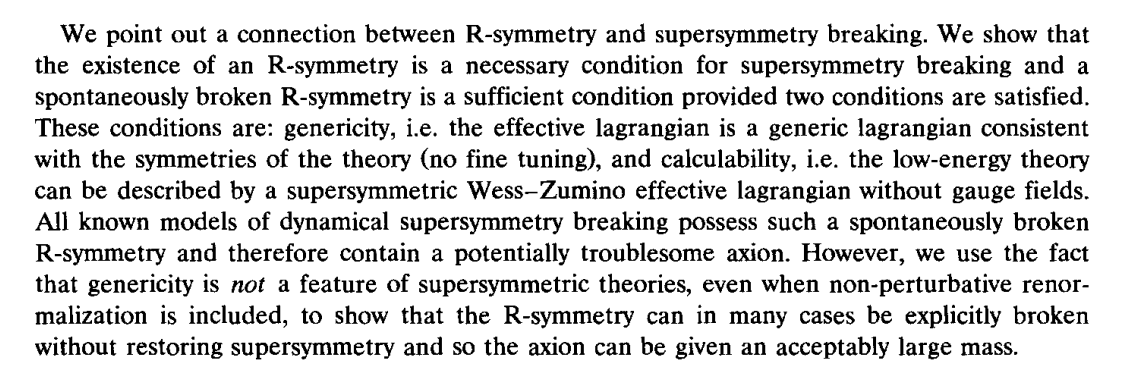
\includegraphics[width=0.8\textwidth]{fig/Nelson1993nfabst.PNG}
  \end{figure}

  \setbeamertemplate{blocks}[rounded][shadow=true]
  \setbeamercolor{block body}{bg=red!10!white, fg=black}
  \begin{block}{}
    \centering
    「\textcolor{DarkMagenta}{R対称性}の破れ」
    $\implies$
    「\textcolor{Goldenrod}{超対称の破れ}」
  \end{block}
  \setbeamertemplate{blocks}[rounded][shadow=true]
  \setbeamercolor{block body}{bg=RoyalBlue!10!white, fg=black}
  \begin{block}{}
    \centering
    「\textcolor{Goldenrod}{超対称の破れ}」
    $\implies$
    「\textcolor{DarkMagenta}{R対称性}の存在」
  \end{block}

\end{frame}

\begin{frame}
  \citeftwo{Nelson:1993nf}{A. E. Nelson and N. Seiberg, Nucl. Phys. B 416 (1994) 46-62.}{R100000002-I027963943}{大河内豊, 超対称性の破れ : 場の理論から弦理論まで, SGC ライブラリ。}

  この例につていは?
  \begin{figure}
    \centering
    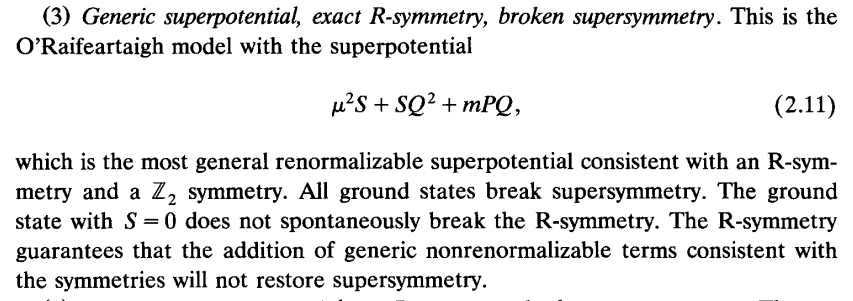
\includegraphics[width=0.8\textwidth]{fig/Nelson1993nf2.PNG}
  \end{figure}
  $S$がflat direction。non-genericな場合に入るのでは。

  また、\cite{R100000002-I027963943}にはこんな記述も。
  \begin{figure}
    \centering
    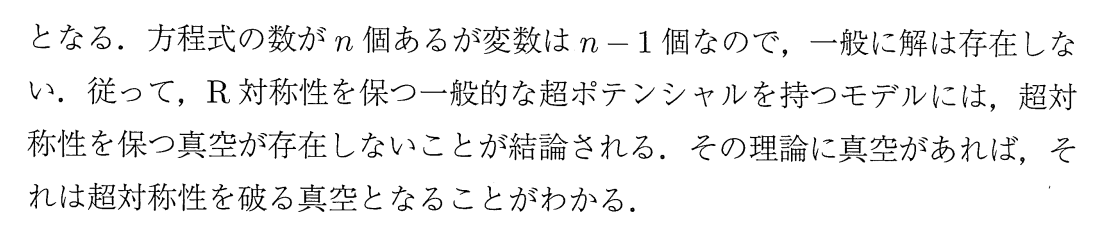
\includegraphics[width=0.8\textwidth]{fig/sgc.PNG}
  \end{figure}

  以下との関係は?
  \setbeamertemplate{blocks}[rounded][shadow=true]
  \setbeamercolor{block body}{bg=red!10!white, fg=black}
  \begin{block}{}
    \centering
    「\textcolor{DarkMagenta}{R対称性}の破れ」
    $\implies$
    「\textcolor{Goldenrod}{超対称の破れ}」
  \end{block}

\end{frame}


\begin{frame}[plain,allowframebreaks]{\eqref{eqn:mX2_Fv}の補足}






\end{frame}





% --------------------------

\section{参考文献}
\begin{frame}[plain,allowframebreaks]{\secname}

  \scriptsize
  \beamertemplatetextbibitems
  \bibliographystyle{ytphys}
  \bibliography{ref}

\end{frame}

\setcounter{framenumber}{\value{Appendix}}
\end{document}
